\documentclass[11pt]{article}
\usepackage[margin=2.5cm]{geometry}
\usepackage{amsmath,amssymb,physics,graphicx}
\title{Chapter 1: Qubits, Gates, Measurement}
\author{Quantum Computing Crash Course}
\date{}
\begin{document}
\maketitle

\section{State}
A qubit is a unit vector $\ket{\psi}=\alpha\ket{0}+\beta\ket{1}\in\mathbb{C}^2$, $\abs{\alpha}^2+\abs{\beta}^2=1$.
Up to global phase,
\begin{equation}
  \ket{\psi}=\cos\tfrac{\theta}{2}\ket{0}+e^{i\varphi}\sin\tfrac{\theta}{2}\ket{1},
  \qquad
  \vec r=(\expval{X},\expval{Y},\expval{Z}).
\end{equation}

\section{Gates}
Gates are unitaries, $U^\dagger U=I$.
\begin{align}
X&=\begin{pmatrix}0&1\\1&0\end{pmatrix}, &
Y&=\begin{pmatrix}0&-i\\i&0\end{pmatrix}, &
Z&=\begin{pmatrix}1&0\\0&-1\end{pmatrix}, &
H&=\tfrac{1}{\sqrt2}\begin{pmatrix}1&1\\1&-1\end{pmatrix}.
\end{align}
Rotations: $R_P(\theta)=e^{-i\theta P/2}=\cos\tfrac\theta2 I-i\sin\tfrac\theta2 P$. Identities: $HZH=X$, $HXH=Z$, $HYH=-Y$.

\section{Measurement}
Born rule: $p(x)=\abs{\braket{x}{\psi}}^2$; post-measurement state $\ket{x}$.
Expectation $\expval{P}{\psi}=p(+1)-p(-1)$; shot-noise error $\sim 1/\sqrt{N}$.

\section{Interference}
For $H\to P(\phi)\to H$ on $\ket{0}$:
\begin{equation}
  \Pr(0)=\cos^2(\phi/2).
\end{equation}

\begin{figure}[h]\centering
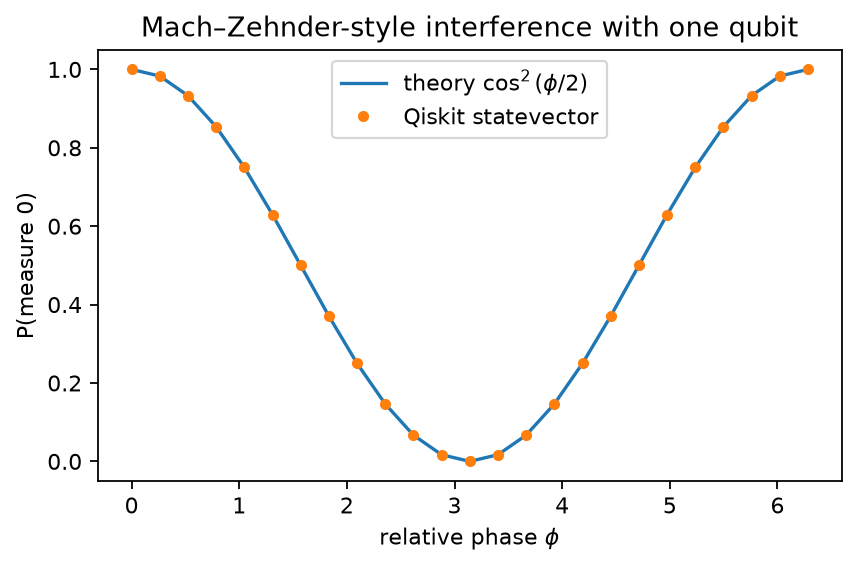
\includegraphics[width=.6\textwidth]{../figures/interference.png}
\caption{Single-qubit interference.}
\end{figure}
\end{document}
